\documentclass[conference]{IEEEtran}
\usepackage{cite}
\usepackage{newtxtext,newtxmath}
\usepackage{amsmath}
\usepackage{graphicx}
\usepackage{booktabs}
\usepackage{xcolor}
\usepackage{tikz}
\usetikzlibrary{arrows.meta,positioning,fit}
\usepackage[hidelinks]{hyperref}
\raggedbottom

\begin{document}

\title{Classification of Gait Activity Using Force Myography}

\author{
\IEEEauthorblockN{Ojaswi Singh}
\IEEEauthorblockA{\small Dept. of Computer Science\\
and Engineering,\\
Amity School of Engineering\\
and Technology,\\
Amity University, Noida, India\\
Email: ojaswis2228@gmail.com}
\and
\IEEEauthorblockN{Mahatva Goel}
\IEEEauthorblockA{\small Dept. of Computer Science\\
and Engineering,\\
Amity School of Engineering\\
and Technology,\\
Amity University, Noida, India\\
Email: goelmahatva@gmail.com}
\and
\IEEEauthorblockN{Roop Singh}
\IEEEauthorblockA{\small Amity Institute of\\
Defence Technology,\\
Amity University,\\
Noida, Uttar Pradesh,\\
India\\
Email: rsingh32@amity.edu}
\and
\IEEEauthorblockN{Ashutosh Tiwari}
\IEEEauthorblockA{\small Centre of Excellence in\\
Affordable Healthcare,\\
Indian Institute of\\
Technology Kharagpur,\\
Kharagpur, India\\
Email: ashutosht@iitkgp.ac.in}
}

\maketitle
\thispagestyle{plain}
\pagestyle{plain}

\begin{abstract}
A control signal is required to control a lower limb assistive device. Current methods use electromyography and mechanical sensors such as inertial measurement units and pressure insoles. This however can be impractical due to the cost and complexity of these techniques. Signals acquired using these techniques suffer from interference due to sweat on the skin, electrode placement and orientation. This paper proposes force myography (FMG). A sensor array is used to capture the volumetric expansion of muscles during locomotion. Eight healthy subjects performed short and long step walking whilst wearing an 8 channel low-cost FMG band on their thighs. Gait activities were classified into six groups: gait initiation, gait termination, short step walking, long step walking, short to long step transition and long to short step transition. Four machine learning classifiers were used to classify subjects not included in training. Classification was also performed for unknown walks of known subjects. When classifying unknown subjects, the support vector machine (SVM) achieved an accuracy of 62.5\% with a balanced accuracy of 55.9\%. The initiation and termination activities were classified with 86\% and 88\% recall. The SVM achieved an accuracy of 90.9\% and balanced accuracy of 80.5\% when classifying known subjects. The short and long steps were classified with 95\% and 93\% recall. The short to long and long to short step transitions were classified with 62\% and 49\% recall. This shows that the thigh FMG band contains the information required to classify gait activities to control an assistive device.
\end{abstract}

\begin{IEEEkeywords}
Force Myography, Gait Activity Classification, Gait Initiation, Gait Termination, Step Length, Prosthetic Control
\end{IEEEkeywords}

\section{Introduction}
To provide impedance and movement control within the joints of a powered lower limb prosthesis/orthosis, it is important to know whether the user is initiating gait, walking at a constant pace, changing their step length or terminating gait. Large weight shifts and muscle activation occur during gait initiation (GI) and gait termination (GT). Step length increases require increased hip flexion/extension and must be supported by the prosthetic knee. Surface electromyography (EMG) has been the most researched signal for locomotion classification [1]--[3]. However, the quality of the signal depends on proper electrode placement and preparation. The signal will be affected by sweating, skin impedance, electromagnetic interference and crosstalk. Inertial measurement units (IMUs) [4] exhibit drift issues, are dependent on the sensor orientation and do not provide information on the muscular activity but instead provide information about the segment motions. Pressure insoles and instrumented footwear provide reliable detection of gait events [5], [6], however they only provide information about the foot--ground interaction after the fact.

Force Myography (FMG) provides measurements of the forces exerted on force-sensitive resistors (FSRs) by the expanding volume of contracting muscles around the limb [7]. As there is no electrical contact with the skin, it is unaffected by sweating and skin impedance, and it is low cost and lightweight. It has been used on the lower limb to detect gait phases and events [8], [9], classify locomotion modes [10]--[12], estimate knee angle [13] and detect short and long steps [14]. However, there has not been any classification of gait initiation, gait termination and step length changes using a single FMG band on the thigh.

This paper makes the following contributions:

\begin{itemize}
\item A low cost FMG band is developed.
\item Important gait activities during locomotion, such as gait initiation, gait termination, step lengths (short and long steps) and step length changes, are classified using only the FMG band.
\item Four different machine learning classifiers are compared on new participants and new walks of known participants. An analysis is also carried out on what sensors are required.
\end{itemize}
\section{Materials and Methods}
Fig.~1 summarises the proposed methodology.

\begin{figure*}[!t]
\centering
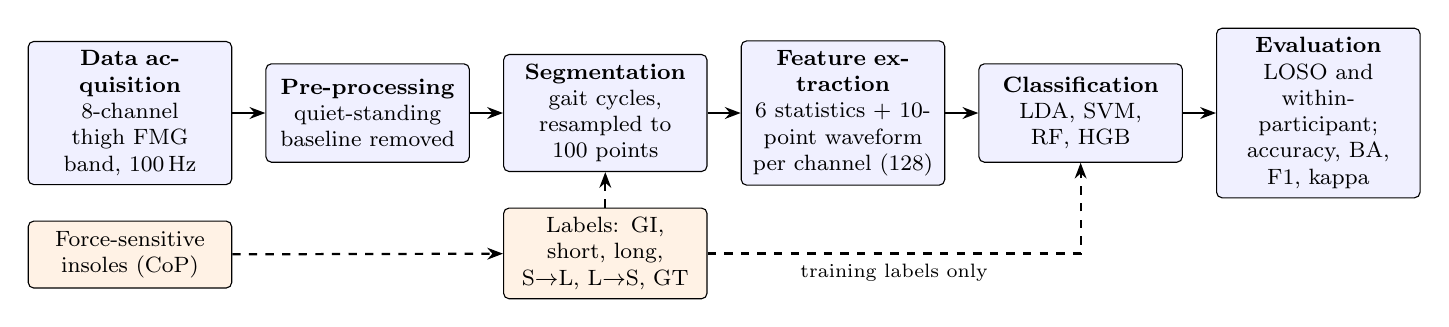
\begin{tikzpicture}[
  box/.style={draw, rounded corners=2pt, align=center, font=\footnotesize, minimum height=1.25cm, text width=2.35cm, fill=blue!6},
  lab/.style={draw, rounded corners=2pt, align=center, font=\footnotesize, minimum height=0.85cm, text width=2.35cm, fill=orange!10},
  arr/.style={-{Stealth[length=2mm]}, thick}, node distance=0.42cm]
\node[box] (a) {\textbf{Data acquisition}\\8-channel thigh FMG band, 100\,Hz};
\node[box, right=of a] (b) {\textbf{Pre-processing}\\quiet-standing baseline removed};
\node[box, right=of b] (c) {\textbf{Segmentation}\\gait cycles, resampled to 100 points};
\node[box, right=of c] (d) {\textbf{Feature extraction}\\6 statistics + 10-point waveform per channel (128)};
\node[box, right=of d] (e) {\textbf{Classification}\\LDA, SVM, RF, HGB};
\node[box, right=of e] (f) {\textbf{Evaluation}\\LOSO and within-participant; accuracy, BA, F1, kappa};
\node[lab, below=0.45cm of a] (g) {Force-sensitive insoles (CoP)};
\node[lab, below=0.45cm of c] (h) {Labels: GI, short, long, S$\to$L, L$\to$S, GT};
\foreach \x/\y in {a/b,b/c,c/d,d/e,e/f} \draw[arr] (\x) -- (\y);
\draw[arr, dashed] (g) -- (h);
\draw[arr, dashed] (h) -- (c);
\draw[arr, dashed] (h.east) -| node[pos=0.25, below, font=\scriptsize]{training labels only} (e.south);
\end{tikzpicture}
\caption{Proposed methodology. Solid arrows show the FMG processing chain. The insole CoP (dashed) is used only to segment and label the data and never enters the classifier.}
\label{fig:flow}
\end{figure*}

\subsection{Participants}
Eight healthy adults (P1--P8) took part in the study. They provided their informed consent in writing. The study was approved by the Institutional Ethics Committee (IEC) at the Indian Institute of Technology Kharagpur (IEC no. IIT/SRIC/DEAN/2025/45).

\subsection{Experimental Setup}
Eight FSRs (FSR400, Interlink Electronics, USA) were attached to pockets made of leather and attached to a flexible strap. This strap was then tightened with an inflexible strap to ensure the sensors would record the whole range of muscle expansion (Fig.~2). The FSRs were placed over the rectus femoris (S1), vastus medialis (S2), between gracilis and adductor longus (S3), adductor magnus (S4), semitendinosus (S5), biceps femoris (S6), iliotibial tract (S7) and vastus lateralis (S8) [10]. Signals were amplified using an MCP6004 (Microchip). The amplified signal was read by an Arduino Nano and transmitted via Bluetooth at a sample rate of 100\,Hz. The force sensitive insoles had sixteen FSRs (FlexiForce A301) [15], which measured the centre of pressure (CoP) and vertical ground reaction force for each foot at a sample rate of 100\,Hz. These were only used to label the data. Each thigh had a band and each shoe had an insole. A push button was used to send a synchronization pulse to both systems at the beginning of each walk.

\begin{figure}[!t]
\centering
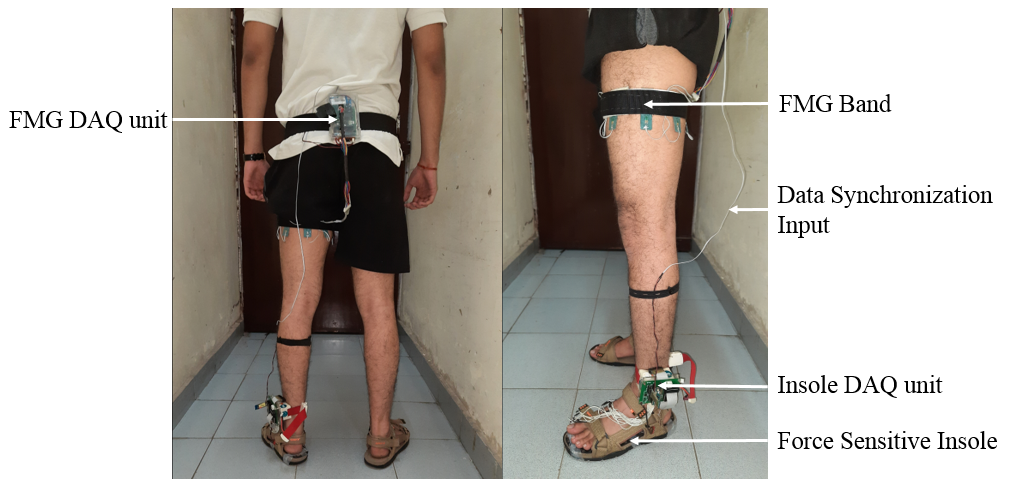
\includegraphics[width=\columnwidth]{figures/participant_setup.png}\\[3pt]
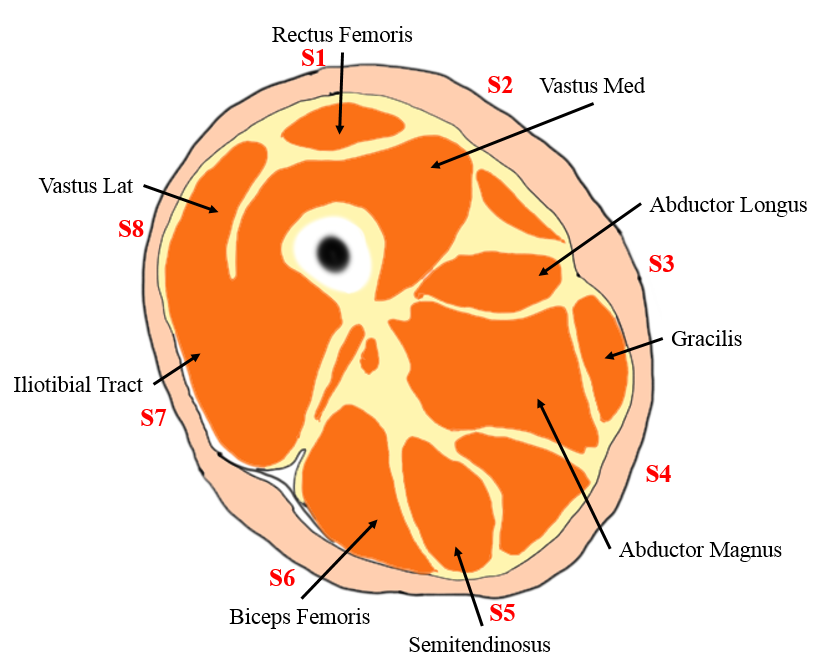
\includegraphics[height=2.45cm]{figures/fsr_placement.png}\hfill
\raisebox{0.75cm}{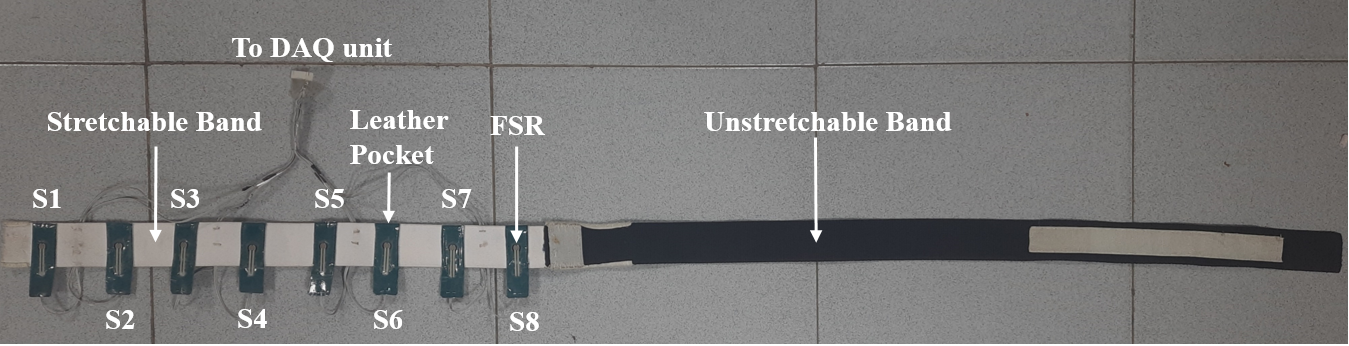
\includegraphics[width=0.6\columnwidth]{figures/fmg_band.png}}
\caption{Top: participant wearing the FMG band, the force-sensitive insole and their data acquisition units. Bottom: sensor placement S1--S8 over the thigh muscles (left) and the FMG band with eight FSRs in leather pockets and the unstretchable outer band (right).}
\label{fig:setup}
\end{figure}

\subsection{Protocol}
Footfall targets were marked on the floor, with large (85\,cm) and small (55\,cm) step lengths. A metronome was used to maintain a steady pace (100 beats per min). The subject walked forward taking five large steps followed by five small steps, then returned to a standing position. The subject then turned around and walked back to the starting position, taking five small steps followed by five large steps. Each participant performed about 40 walks; 331 walks were analysed (39--48 per participant), and each limb was analysed separately.

\subsection{Segmentation and Labelling}
A segment cut was identified for each limb from its own CoP (Fig.~3). CoP data have a minimum (valley) corresponding to each contact of the foot. Therefore, a gait cycle can be identified between two consecutive valleys for a given limb. We denote by $r$ the rise from the quiet standing phase, and $v_{0}$,...,$v_{11}$ the first twelve valleys. For each limb, this provided 12 examples: GI from $r$ to $v_{1}$, cycles 2--5 and 7--11 (short/long steps), cycle 6 (transition S$\to$L or L$\to$S), and GT from $v_{11}$ to rest. On the one trial with hand marks from an expert, the automatic cuts agreed with the marks within 50\,ms. The direction of each walk (short-to-long or long-to-short) was determined by the excursion of CoP, which is larger during long step cycles. All 612 consecutive pairs of walks alternated, as required by the protocol. Of 672 limb recordings, 627 were segmented. Examples using estimated samples (gap filled) were removed giving 7196 examples: 570 GI, 2670 short, 2753 long, 300 S$\to$L, 306 L$\to$S and 597 GT.

\begin{figure}[!t]
\centering
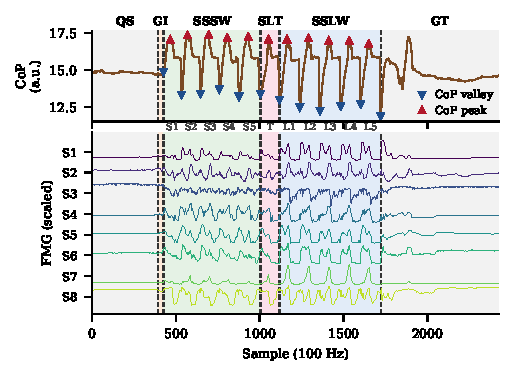
\includegraphics[width=\columnwidth]{figures/fig1_segmentation.pdf}
\caption{Segmentation of one short-to-long walk (P8, left limb). Triangles mark CoP valleys (foot contact) and peaks; dashed lines are $r$, $v_{0}$, $v_{5}$, $v_{6}$ and $v_{11}$. Only the eight FMG channels (bottom) are classifier input.}
\label{fig:seg}
\end{figure}

\subsection{Feature Extraction}
The static baseline (median of the 0.5\,s preceding $r$) was subtracted from the FMG signal of each example, which was then resampled to 100 samples. Six statistical features were extracted per channel: mean, standard deviation, RMS value, 10th--90th percentile range, mean absolute successive difference and linear slope. Additionally, the waveform was sampled at 10 evenly spaced intervals resulting in a total feature set size of 128. The feature set was also tested using only the 48 statistics, and with the cycle length added. The features were normalized using the median and interquartile range of the training data.

\subsection{Machine-Learning Classifiers}
Four classification algorithms were implemented using scikit-learn [16]. All hyperparameters were specified prior to testing. Linear discriminant analysis (LDA) makes the assumption that each class follows a Gaussian distribution and that all classes have a common covariance matrix. A shrinkage method was applied to the covariance estimate, using the Ledoit-Wolf method. The support vector machine (SVM) creates a non-linear mapping of the features using an RBF kernel function $K(\mathbf{x},\mathbf{x}')=\exp(-\gamma\lVert\mathbf{x}-\mathbf{x}'\rVert^2)$ with $\gamma$ being scaled according to the variance of the features. The resulting hyperplane is found by maximising the margin of separation between classes ($C=10$). A one vs one approach was used to separate the 6 classes into 15 binary SVMs. The random forest (RF) algorithm performs classification based on the predictions of 300 decision trees. Each tree is trained on bootstrapped samples of the data. At each split only $\sqrt{d}$ features are considered as candidates. The histogram gradient boosting (HGB) algorithm performs sequential boosting by building an ensemble of 300 trees with a maximum of 31 leaves and learning rate of 0.1. Each tree helps to correct the mistakes made by previous trees. Class weights were set to be inversely proportional to the number of samples in each class for all four algorithms.

\subsection{Evaluation}
For leave-one-subject-out (LOSO) evaluations all walks from a single participant were used for testing simulating a new user [17]. For within subject evaluations the data was split using 5-fold cross-validation, so that each complete walk was contained within a single fold. Accuracy, balanced accuracy (BA), macro-F1, per class precision, recall, F1 score and Cohen's kappa were calculated. BA and macro-F1 were reported as the mean $\pm$ standard deviation over participants.

\section{Results}
Table~I shows the performance of the different classifiers. It can be seen that using waveform features improved performance by between 8 and 11 percentage points. The SVM classifier performed best with a balanced accuracy of 55.9\% for unseen users and 80.5\% for known users. Adding cycle time gave little benefit.

\begin{table}[!t]
\caption{Balanced Accuracy (BA) and Macro-F1 in \%, Mean $\pm$ SD over Participants}
\label{tab:t1}
\centering
\setlength{\tabcolsep}{4pt}
\begin{tabular}{llcc}
\toprule
Features & Model & BA & Macro-F1 \\
\midrule
\multicolumn{4}{l}{\emph{Unseen participants (LOSO)}} \\
48 statistics & LDA / SVM & 37.6 $\pm$ 4.9 / 45.0 $\pm$ 6.5 & 35.0 / 37.3 \\
 & RF / HGB & 42.2 $\pm$ 7.0 / 45.1 $\pm$ 5.9 & 39.9 / 40.5 \\
128 features & LDA & 47.5 $\pm$ 7.6 & 44.8 $\pm$ 8.8 \\
 & SVM & \textbf{55.9 $\pm$ 8.6} & 51.1 $\pm$ 9.1 \\
 & RF & 51.8 $\pm$ 6.7 & 49.1 $\pm$ 8.5 \\
 & HGB & 55.0 $\pm$ 8.6 & 51.3 $\pm$ 10.9 \\
+ duration & SVM / HGB & 57.5 $\pm$ 8.1 / 57.3 $\pm$ 7.8 & 53.1 / 53.7 \\
\midrule
\multicolumn{4}{l}{\emph{Unseen walks of known participants}} \\
128 features & LDA & 75.7 $\pm$ 6.0 & 77.2 $\pm$ 6.2 \\
 & SVM & \textbf{80.5 $\pm$ 6.5} & \textbf{81.6 $\pm$ 6.4} \\
 & RF & 66.1 $\pm$ 4.1 & 67.0 $\pm$ 5.4 \\
 & HGB & 74.0 $\pm$ 5.8 & 76.1 $\pm$ 6.8 \\
\bottomrule
\end{tabular}
\end{table}

Table~II and Fig.~4 show the classifier has good recall for gait start and end events but poor recognition of transitions.

\begin{table}[!t]
\caption{Per-Class Precision (P), Recall (R) and F1 of the SVM in \%}
\label{tab:t2}
\centering
\setlength{\tabcolsep}{3.5pt}
\begin{tabular}{lcccccc}
\toprule
 & \multicolumn{3}{c}{Unseen participants} & \multicolumn{3}{c}{Known participants} \\
\cmidrule(lr){2-4}\cmidrule(lr){5-7}
Class & P & R & F1 & P & R & F1 \\
\midrule
GI & 62.0 & 86.0 & 72.1 & 92.2 & 94.9 & 93.5 \\
Short step & 78.0 & 56.7 & 65.7 & 94.5 & 95.2 & 94.8 \\
Long step & 72.5 & 67.0 & 69.6 & 92.1 & 93.4 & 92.8 \\
S$\to$L transition & 17.7 & 21.0 & 19.2 & 73.3 & 62.3 & 67.4 \\
L$\to$S transition & 11.9 & 19.9 & 14.9 & 50.5 & 48.7 & 49.6 \\
GT & 49.8 & 88.1 & 63.6 & 94.8 & 92.0 & 93.4 \\
\midrule
Accuracy / kappa & \multicolumn{3}{c}{62.5 / 0.49} & \multicolumn{3}{c}{90.9 / 0.87} \\
\bottomrule
\end{tabular}
\end{table}

\begin{figure}[!t]
\centering
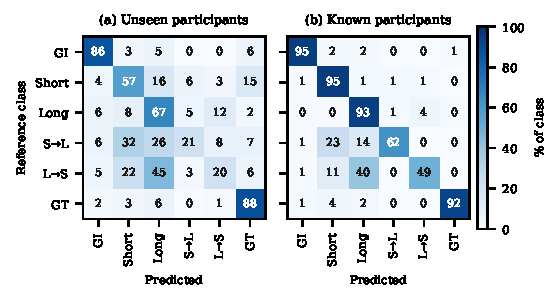
\includegraphics[width=\columnwidth]{figures/fig_confusion.pdf}
\caption{Row-normalised confusion matrices (\%) of the SVM: (a) unseen participants (LOSO), (b) unseen walks of known participants.}
\label{fig:confusion}
\end{figure}

Removing medial sensors gave little effect (Table~III). Using only sensor S7 gave reasonable performance (Table~III). Using only the lateral sensor S7 gave similar performance to using the whole sensor band (55.5\% vs 55.9\%) for unseen users. The training time was 1.0\,s per fold and classification took only 0.3\,ms per gait cycle on a laptop CPU.

\begin{table}[!t]
\caption{Balanced Accuracy (\%) of the SVM with Sensor Subsets}
\label{tab:t3}
\centering
\setlength{\tabcolsep}{4pt}
\begin{tabular}{lcc}
\toprule
Sensors & Unseen & Known \\
\midrule
All eight (S1--S8) & 55.9 & \textbf{80.5} \\
Without medial (S3, S4) & \textbf{56.4} & 80.1 \\
Without anterior (S1, S2, S8) & 53.1 & 79.1 \\
Without posterior (S5, S6) & 53.4 & 78.3 \\
Lateral S7 only & 55.5 & 69.8 \\
\bottomrule
\end{tabular}
\end{table}

\section{Discussion}
Classification of initiation and termination was good even for new users. This was due to the clear differences in muscular deformation between the initiation/termination periods and the rhythmic movement. Short and long steps could be reliably differentiated within subjects (93--95\% recall) however were more difficult to differentiate between subjects (57--67\%). This suggests that the variation in FMG between different step lengths is due to personal factors such as muscle volume and positioning of band. A short calibration period for the user should largely compensate for this difference. The transitions were the most difficult to classify. There was only one transition cycle per walk, with characteristics similar to the neighbouring steps. The results from analysing the sensor data suggest that the number of sensors can be reduced to reduce the size of band with little reduction in performance. This, along with a prediction time of 0.3\,ms, supports use in an embedded system. Limitations to this research include only having 8 healthy subjects, only one cadence and only on level ground. The gait cycles were cut using insole data which would need to be replaced by online detection in a real device.

\section{Conclusion}
An eight channel low cost thigh FMG band was able to classify gait onset and gait offset with a recall of 86--88\% in participants not used in training. When using training data from the same user, the model achieved an accuracy of 90.9\% across 6 gait activities. Further work will be done with transfemoral amputees, varying speeds and terrains. Real time classification will also be investigated for use in prosthetic control.

\begin{thebibliography}{00}
\bibitem{r1} H. Huang, F. Zhang, L. J. Hargrove, Z. Dou, D. R. Rogers, and K. B. Englehart, ``Continuous locomotion-mode identification for prosthetic legs based on neuromuscular--mechanical fusion,'' \emph{IEEE Trans. Biomed. Eng.}, vol. 58, no. 10, pp. 2867--2875, 2011.
\bibitem{r2} D. Joshi, B. Nakamura, and M. E. Hahn, ``High energy spectrogram with integrated prior knowledge for EMG-based locomotion classification,'' \emph{Med. Eng. Phys.}, vol. 37, no. 5, pp. 518--524, 2015.
\bibitem{r3} D. Joshi and M. E. Hahn, ``Terrain and direction classification of locomotion transition using neuromuscular and mechanical input,'' \emph{Ann. Biomed. Eng.}, vol. 44, no. 4, pp. 1275--1284, 2016.
\bibitem{r4} A. J. Young, A. M. Simon, N. P. Fey, and L. J. Hargrove, ``Intent recognition in a powered lower limb prosthesis using time history information,'' \emph{Ann. Biomed. Eng.}, vol. 42, no. 3, pp. 631--641, 2014.
\bibitem{r5} A. Tiwari and D. Joshi, ``An infrared sensor-based instrumented shoe for gait events detection on different terrains and transitions,'' \emph{IEEE Sensors J.}, vol. 20, no. 18, pp. 10779--10791, 2020.
\bibitem{r6} A. Tiwari, A. Pai, and D. Joshi, ``A shoe-mounted infrared sensor-based instrumentation for locomotion identification using machine learning methods,'' \emph{Measurement}, vol. 168, Art. no. 108458, 2020.
\bibitem{r7} Z. G. Xiao and C. Menon, ``A review of force myography research and development,'' \emph{Sensors}, vol. 19, no. 20, Art. no. 4557, 2019.
\bibitem{r8} X. Jiang, K. H. T. Chu, M. Khoshnam, and C. Menon, ``A wearable gait phase detection system based on force myography techniques,'' \emph{Sensors}, vol. 18, no. 4, Art. no. 1279, 2018.
\bibitem{r9} A. K. Godiyal, H. Verma, N. Khanna, and D. Joshi, ``A force myography-based system for gait event detection in overground and ramp walking,'' \emph{IEEE Trans. Instrum. Meas.}, vol. 67, no. 10, pp. 2314--2323, 2018.
\bibitem{r10} A. K. Godiyal, M. Mondal, S. D. Joshi, and D. Joshi, ``Force myography based novel strategy for locomotion classification,'' \emph{IEEE Trans. Human-Mach. Syst.}, 2018, doi: 10.1109/THMS.2018.2860598.
\bibitem{r11} A. K. Godiyal, U. Singh, S. Anand, and D. Joshi, ``Analysis of force myography based locomotion patterns,'' \emph{Measurement}, vol. 140, pp. 497--503, 2019.
\bibitem{r12} A. K. Godiyal and D. Joshi, ``Optimal force myography placement for maximizing locomotion classification accuracy in transfemoral amputees: A pilot study,'' \emph{IEEE J. Biomed. Health Inform.}, 2020, doi: 10.1109/JBHI.2020.3015317.
\bibitem{r13} A. Kumar, A. K. Godiyal, P. Joshi, and D. Joshi, ``A new force myography-based approach for continuous estimation of knee joint angle in lower limb amputees and able-bodied subjects,'' \emph{IEEE J. Biomed. Health Inform.}, 2020, doi: 10.1109/JBHI.2020.2993697.
\bibitem{r14} R. Khatavkar, A. Tiwari, R. Bajpai, and D. Joshi, ``Gait step length classification using force myography,'' in \emph{Proc. Int. Conf. Advancement in Technology (ICONAT)}, 2022, pp. 1--4.
\bibitem{r15} A. Tiwari and D. Joshi, ``Template-based insoles for the center of pressure estimation in different foot sizes,'' \emph{IEEE Sensors Lett.}, vol. 4, no. 8, pp. 1--4, 2020.
\bibitem{r16} F. Pedregosa \emph{et al.}, ``Scikit-learn: Machine learning in Python,'' \emph{J. Mach. Learn. Res.}, vol. 12, pp. 2825--2830, 2011.
\bibitem{r17} S. Saeb, L. Lonini, A. Jayaraman, D. C. Mohr, and K. P. Kording, ``The need to approximate the use-case in clinical machine learning,'' \emph{GigaScience}, vol. 6, no. 5, pp. 1--9, 2017.
\end{thebibliography}

\end{document}
